\documentclass[11pt]{article}
\usepackage[margin=1in]{geometry}
\usepackage[parfill]{parskip}
\usepackage{graphicx}
\usepackage{amssymb}
\usepackage[colorlinks=true,
						linkcolor=red,
						urlcolor=red,
						citecolor=blue,
						anchorcolor=blue]{hyperref}
\usepackage{subcaption}

\title{OPT: Optical Pumping}
\author{UC Berkeley Advanced Lab}
\date{}

\begin{document}
\maketitle
\section{Description}
This experiment is quantum mechanics in action. When a sample of gaseous atoms is placed in a static magnetic field, the electronic states undergo Zeeman splitting in addition to fine-structure and hyperfine-structure splittings. By applying polarized light at the proper frequency, we can induce transitions from ground state levels to excited state energy levels. The atoms then decay to higher ground state levels until we have ``pumped" all of them into the same (highest) ground state energy level. At this point we can see an increase in light passing through the sample because no more can be absorbed. However, when we apply a radiofrequency signal of just the right energy to stimulate transitions to a lower level, we see a sudden decrease in the radiation signal as the system is again pumped to the higher level. By determining the frequency of the RF signal we gain information about the atomic energy levels.

You will need to use your knowledge of fine, hyperfine, and Zeeman splitting to find the energy levels of two isotopes of rubidium. You will determine the nuclear spins of the isotopes, and the strength of the earth's magnetic field in the laboratory.

\begin{center}
\fbox{This lab will be graded 20\% on theory, 30\% on technique, and 50\% on analysis.}
\end{center}

\section{Before the 1st day of Lab}
\begin{enumerate}
\item View the \href{http://youtu.be/v4StxGAhm8Y}{Optical Pumping video}. Make sure you also complete the quiz (found under the Assignments tab on bCourses).

Some notes about common misconceptions from the video:
\begin{itemize}
\item \textbf{05:26} The $^2$P$_{3/2}$ state splits into $F=3,2,1,0$ because $J=I=3/2$ for $^{87}$Rb.
\item \textbf{06:30} The order of the $m_F$ sublevels of the $F=1$ state has to be reversed because $g_F=-1/2$
\item \textbf{12:34} The ratio of probabilities is not generally 50:50; it depends on the specific sublevels involved. This does not make too much of a difference for the discussion.
\item \textbf{13:05} In the OPT experiment, th atoms are actually pumped into an $|m_F|=2$ sublevel of the $F=2$ state in the case of $^{87}$Rb
\item \textbf{14:53} Some would say it is wrong to call radio-frequency radiation ``light"
\item \textbf{18:02} It is incorrect to label the horizontal axis $t$
\item \textbf{20:22} The filter that removes the $D_2$ radiation is note there to get rid of noise. In fact, if one removes the filter, while the same ground state will be pumped, the pumping, however, will not result in the rubidium vapor becoming transparent. This is a finer point of the experiment (of which there are many, most of them being glossed over).
\end{itemize}

\item Note that \href{http://experimentationlab.berkeley.edu/optprelab}{Check Points} are examination points that are placed in this lab where you must stop and call a GSI or professor to make sure you understand what's expected. There could  be multiple check points throughout your lab so make sure you don't skip them since there is a sign off sheet that must be turned in with your lab report. There are 3 Checkpoints in this lab.

\item Complete the \href{http://experimentationlab.berkeley.edu/optcheckpoints}{OPT Prelab}. Read through the lab manual and the references to prepare answers to the prelab questions. Discuss the experiment and pre-lab questions with any faculty member or GSI and get it signed off by that faculty member or GSI. Turn in the signed pre-lab sheet with your lab report.

\end{enumerate}

\section{Suggested Reading}
The following resources should help you answer the prelab questions (Ramsey 1953 is particularly useful for deriving the Breit-Rabi equation). Definitions of some terms that you should be familiar with can be found \href{http://experimentationlab.berkeley.edu/definitionsopt}{here}.
\begin{itemize}
\item \href{http://physics111.lib.berkeley.edu/Physics111/Reprints/OPT/05-Optical_Pumping-DeZafra.pdf}{R.L. De Zafra, ``Optical Pumping", Amer. Journ. of Phys. 28, 646 (1960). QC1.A4}
\item \href{http://experimentationlab.berkeley.edu/sites/default/files/images/OPT_RbEnergyLevels.pdf}{Reference Rubidium Diagrams Rb Energy Levels}
\item \href{http://physics111.lib.berkeley.edu/Physics111/Reprints/OPT/02-Optical_Pumping-Bloom.pdf}{A.L. Bloom, ``Optical Pumping", Scientific American, October 1960, p.72. T1.S5}
\item \href{http://physics111.lib.berkeley.edu/Physics111/Reprints/OPT/06-Experiment_7.pdf}{Experiment 7 report on Optical Pumping}
\item \href{http://physics111.lib.berkeley.edu/Physics111/Reprints/OPT/04-Nuclear_Moments.pdf}{N.F. Ramsey, Nuclear Moments, Wiley, 1953. QC174.1.R31.}
\item \href{http://physics111.lib.berkeley.edu/Physics111/Reprints/OPT/OPT%20Rubidium.pdf}{C.E. Moore. ``Rubidium." Atomic Energy Levels Vol. II, National Bureau of Standards, 1952. QC453.M6}
\end{itemize}

\section{Objectives}
\begin{itemize}
\item Optical Pumping of Rubidium Atoms, Rb85 and Rb87; measurement of the nuclear spins
\item Explore Magnetic Hyperfine Interactions of Rubidium
\item Observe Zero-Field Transitions
\item Confirm Breit-Rabi Equation
\item Observe Double Quantum Transitions
\item Study Rabi Oscillations 
\item Measure Optical Pumping pump up and pump down Times
\item Study Temperature Dependence of Atomic Parameters
\item Navigate through the DS345 Function Generator 
\item Measure the Energy Differences and Find Resonance Between Zeeman Splitting of Atomic Systems
\item Determine the Nuclear Spins of Isotopes 
\item Measure the value of the earth's magnetic field at UC Berkeley and angle at the Lab.
\end{itemize}

\section{Experimental Procedure}
Taking data for this experiment is more straightforward than for any other lab in this course. But the experiment deserves more time and thought than most because it illustrates fundamental ideas about quantum mechanics which you probably have only vague notions. Take the time to think about what's going on, and answer any questions that occur to you. You should know the equipment and how this experiment is connected to make things work. If you understand the signal flow for this experiment then it will be easy to complete.

\subsection{Getting started}
Look over the block diagram Fig. \ref{fig:diag} and check the connections of the equipment carefully.  Make sure you understand what each unit does and that you know the limitations of the equipment (e.g. don't run the current of the coil higher than 3 A; be sure to understand how the voltmeter and shunt gives you precise current measurements; don't drive the RF at more than 5 V; don't heat the bulb over 50$^\circ$C; etc.).  Inspect and open carefully the Rb light box to see its construction. You can get a better understanding of how the bulb works through the tutorial video and the definitions page. Be particularly careful of the D$_1$ pass filter. It is expensive to replace! All pieces in this unit are already in their proper places. 

\begin{figure}
\centering
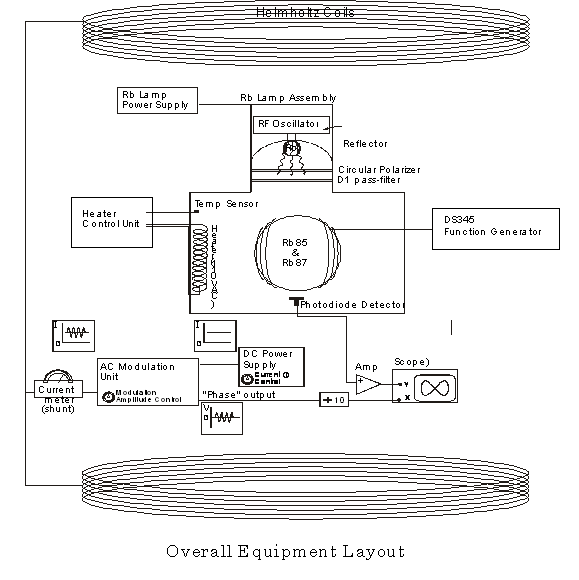
\includegraphics[width=\textwidth]{figures/OPTimage001.png}
\caption{Equipment block diagram}
\label{fig:diag}
\end{figure}

You will find a large glass bulb in the light box, placed between the Rb lamp and the photodetector. The glass bulb is a Rubidium ABS Cell, Pyrex 80 mm OD sphere filled with Rb + 20 Torr N$_2$ (filled with a thin atomic gas of rubidium in both its naturally abundant isotopes ($^{85}$Rb and $^{87}$Rb). Rb also resides on the walls of the glass bulb, whence it can be released by heating the glass cell, thereby giving a stronger optical pumping signal. The bulb also contains an inert buffer gas (e.g. helium, neon, or molecular nitrogen). The buffer gas keeps the Rb atoms localized within the volume of the bulb for long times before they diffuse onto the glass walls of the bulb. The bulb may or may not be coated with a thin wax layer (paraffin). The wax keeps the Rb atoms from hitting the glass surface, allowing them to retain their spin polarization for longer, and thereby leading to a longer relaxation time from the optically pumped state.

\textbf{The glass bulbs are fragile, expensive, and hard to replace. You should not need to handle the bulb or remove it from the light box. If you feel you need to do this, then please ask one of the laboratory teaching staff for help.}

Turn on all the equipment, starting with the Main switch (lower right-hand corner of the Rubidium Lamp Supply/Coil Driver Panel). Set the Rubidium Supply Output Current for the Rb lamp to approximately 25 milliamperes using the Adjust Knob. (Like much of the experimental apparatus, the Rb lamps at the two Optical Pumping stations are not identical; one may require a higher current to light the lamp [perhaps 30 mA].)

\textbf{Never turn off the plug strip if any of the equipment is powered up.}

When you turn on the SR560 Voltage Pre-amp (Fig. \ref{fig:preamp}) make sure that the INPUT `A' is selected, the DC/GND/AC button is set to the AC position. To start, set the Gain to 500, LF Roll-off to 0.1 Hz, and the HF Roll-off to 10 KHz. You may have to change some settings to make your signal clear. Also note that if you suddenly lose your signal, i.e. if your scope trace goes to a flat-line, you should press the OL REC (OverLoad RECovery) button. The SR560 requires you to adjust the dynamic reserve and the filter roll-off; set the gain mode to low noise and the roll off to 6 dB per octave for both the high and low pass filters. 

\begin{figure}
\centering
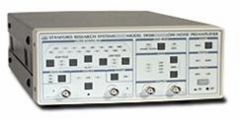
\includegraphics{figures/OPTimage002.jpg}
\caption{SR560 preamplifier}
\label{fig:preamp}
\end{figure}

\subsection{Understanding the function generator}
We will be using a DS345 synthesized function generator to drive the RF coils in this experiment. Before you begin taking data, it would be wise to familiarize yourself with its capabilities, its limitations, and its interface.

\begin{figure}
\begin{subfigure}{0.5\textwidth}
	\centering
	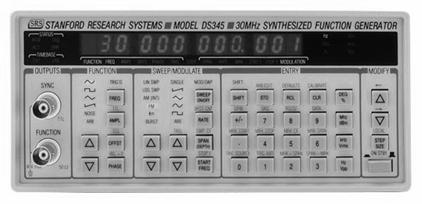
\includegraphics[width=0.8\linewidth]{figures/OPTimage004.jpg}
	\caption{Front panel}
\end{subfigure}
\begin{subfigure}{0.5\textwidth}
	\centering
	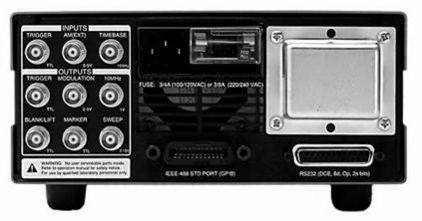
\includegraphics[width=0.8\linewidth]{figures/OPTimage005.jpg}
	\caption{Back panel}
\end{subfigure}
\caption{DS345 synthesized function generator}
\label{fig:funcgen}
\end{figure}


Try experimenting with the signal modulation capabilities of the DS345. Connect the modulation output (not terminated) of the DS345 (on the back panel, see Fig. \ref{fig:funcgen}) to the Ch. 1 (X) input of the oscilloscope and connect the terminated function output of the DS345 to the Ch. 2 (Y) input of the scope. Set the oscilloscope to trigger off of channel 1 in the ``Norm" mode. Set the scope to ``Alt" rather than ``Chop". Experiment with different amplitude modulation waveforms, span, and rate settings on the DS345. You might also try using the X-Y mode of the scope to observe the output of the DS 345 (function output against modulation output) but don't let it confuse you. It is important to have a clear understanding of what the X-Y mode represents and when to use it.

Now try frequency modulation. Note that you can't set the span to twice the carrier frequency or more (the DS345 has trouble making oscillations with zero or negative frequencies). Try different modulation waveforms; look at sine, triangle and ramp modulations. Again, start with the oscilloscope in the linear, time sweep mode. The X-Y mode can also be revealing if you keep in mind what the modulation output represents. As with AM, in FM, the modulation output gives a 0-5 V representation of the modulation function. Again, zero volts corresponds to the minimum frequency (the carrier frequency minus half the span) and 5 volts corresponds to the maximum frequency (the carrier frequency plus half the span), and so forth. You should now have familiarized with the DS345 enough for this experiment.

\fbox{
\parbox{0.97\linewidth}
{\textbf{This is a Checkpoint}: Once you feel you are familiar with the DS345, call over a GSI or Professor and explain what you will be using it for in this lab and show them you are cable of navigating the device.}
}

\subsection{Effect of temperature on signal strength}
The temperature controller provides a DC signal to copper wires located inside the apparatus next to the rubidium bulb. The electrical current will radiate in the form of heat from the wires. You will notice that the "DC microamp" display of the controller runs both ways. In order to increase the heat you will want to turn the black knob clockwise, shifting the red needle to the left. The greater the displacement of the needle the faster the temperature will rise, you will be able to keep your signal at roughly a constant temperature by adjusting this knob. 

Heat the sample to 48$^\circ$C, then turn the heater off to reduce noise, but remember that you want the temperature between 38$^\circ$C and 45$^\circ$C for good data (You will explore this temperature dependence in the following section and the noise associated with it). A reading from the temperature sensor is output to an LED display labeled 'Oven Temperature'. Make sure the temperature does not go above 55$^\circ$C; if you start to approach this temperature, turn down the thermostat. The heater has an over-temperature shutoff switch in the heater box. If you over heat the box it will need time to rest and you should call one of the staff.

As mentioned before, heating the glass cell will release more rubidium atoms off the walls of the cell and into the buffer gas in the volume of the cell. The higher vapor density will attenuate the Rb lamp more when it is not optically pumped, and so your detected signal -- the difference in optical transmission through the cell in the presence and the absence of optical pumping -- will be larger. However, as the cell heats up and the vapor density increases, there may be effects, such as Rb-Rb collisions, that reduce the lifetime of the optically pumped electronic state, having the effect of decreasing the strength of your signal.

Take an experimentalist's approach: once you have identified the optical pumping resonance of each of the two isotopes in the following section, explore the variations of the signal with the changing temperature of the cell over the allowed range (from room temperature up to about 55$^\circ$C as shown below). See what effect this has on the resonance strength and whether or not the value of resonance changes with temperature. The effect may be different for the two rubidium isotopes. 

\begin{figure}
\centering
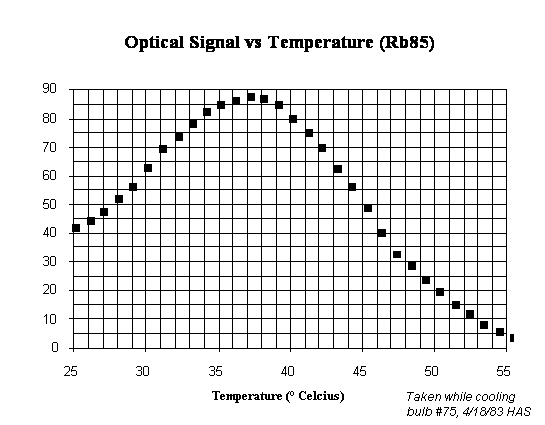
\includegraphics[width=\textwidth]{figures/OPTimage006.png}
\caption{An example plot of signal strength as a function of bulb temperature for $^85$Rb. Note that the peak temperature for $^87$Rb may be different.}
\label{fig:tempdep}
\end{figure}

\subsection{Finding resonance}
\subsubsection{Using the function generator}
The setup will need to be slightly tuned to find the resonance frequencies of the two isotopes. Initially we will want to induce the Zeeman splitting by driving a DC current through the magnetic coil, power the coils with roughly 1.0 Amp to start with. The strength of the coils will change the spacing between Zeeman levels and will ultimately dictate the resonance frequency needed to induce stimulated emission of the Rb. Next the RF coils shold be set to create the electromagnetic radiation required to induce these emissions. They can be driven using the function output of the DS345. The variation in the opacity of Rubidium gas that occurs when it is optically pumped and then hit by the resonance frequency electromagnetic radiation can be observed through the photodiode. In order to read the signal generated inside the bulb the photo diode's output will need to be connected to the PRE-AMP as the signal of radiation will be very low. It is important to make sure the PRE-AMP settings are as specified before or you will not receive a proper signal. Finally run the output of the PRE-AMP (the amplified photo diode output) to Ch.2 (Y) of the oscilloscope and keep Ch.1 (X) connected to the DS345's modulation output. It will be best to observe the results in the X-Y mode of the oscilloscope. 

Use the Current knob on the Power Supply to adjust the current and the 10m$\Omega$ shunt to measure it. Current shunt resistors are low resistance precision resistors used to measure AC or DC electrical currents by the voltage drop those currents create across the resistor. The shunt is a calibrated resistor and is temperature compensated so that its resistance value does not change with a change in temperature (On average the shunt's resistance changes less than 0.002\% (or 20 ppm = parts per million) per $^\circ$C of temperature change). The voltage that develops across the shunt is 10 mV per amp of current through the coils. The digital volt meter reads the millivolt reading. (Note that there is a button on the front of the Digital Volt meter that changes the connections from front to rear of the unit.) This button should be in the front position. A circuit diagram of the set up can be found \href{http://experimentationlab.berkeley.edu/sites/default/files/OPT/Circuitformagnetic%20coils.png}{here}.
Make a note of the current value that the multimeter and the power supply give you (the Multimeter displays voltage drop and will have to be converted to current using ohms law). 

On the oscilloscope, with the modulation connected to Ch.1 and the amplified signal connected to Ch.2, you should see something like what is shown in Fig. \ref{fig:funcgen_res}. You may see some 60 Hz noise in your signal; adjusting the connections may help minimize the problem. The fault may simply be related to the electronics and not the settings. It is important to recognize the source of this noise if it arises (60 Hz noise is a commonly recurring theme in experimental physics). The function of the modulated signal will ultimately dictate how the oscilloscopes depicts what is happening. Since the frequency modulation serves to sweep a range set by the span of the function generator and output frequencies ranging from Out$_F-$Span$/2$ to Out$_F+$Span$/2$ the oscilloscope in XY mode will divide this frequency range amongst roughly 10 divisions along the axis where the Modulation output of the function generator is plugged in starting (with the minimum frequency on the left hand side of the display). Based on this information it should be noted that the span can not be equal to or greater than twice the carrier frequency of the function output [In case the reasoning behind this isn't so obvious see the  FM Modulation section in the DS345 Manual]. This, in combination with understanding what the perpendicular axis represents in the XY plot, is useful for determining what the resonance frequencies of the isotopes are. Center the output of the function generator to a frequency close to one that would correspond to the energy difference between two Zeeman levels (You can calculate what this energy difference would be by using the Breit-Rabi equation you found in the prelab), thus inducing spontaneous emission. The signal should be a sine wave with a 10 Hz modulation. Sweep a range you believe will hold the resonance frequencies for the two isotopes, if you have hit the resonance frequency then the figure should look like figure 4. Once you have found the proper range it will be possible to better resolve the image to extract a better estimate of the resonance frequency value. You should ebe able to determine which peak corresponds to which isotope by examining the natural abundance of the two isotopes. 

\begin{figure}
\centering
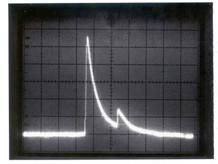
\includegraphics{figures/OPTimage003.jpg}
\caption{Amplified photodiode signal with large span frequency modulation.}
\label{fig:funcgen_res}
\end{figure}

\subsubsection{Using the Helmholtz coils}
As explained in the introduction video, modulating the magnetic field of the Helmholtz coils is a quicker and more accurate way of finding what the resonance frequency is. That is, we will modulate the coil current and not the RF. The magnetic modulation does not cover as much as the RF modulation did so change the frequency of the carrier so it is closer to the resonance. Turn on field modulation by flipping the ``Field" switch on the Coil Driver panel, and turn on the ``Phase Out" output with the ``Phase Switch".

Familiarize yourself with the Coil Driver panel: The Phase Adjust control on Coil Driver panel changes the phase of the modulation signal seen by the scope (the Phase Out signal) relative to the modulation signal that the rubidium sample experiences (which is the actual modulation in the coil current that changes the phase of the photo-detected signal). Connect the Phase out signal to Ch 1 (X) of the oscilloscope and the amplified photodetector signal to Ch 2 (Y). With the scope in Dual Trace Mode (both channels), trigger on EXT/Line Source (60 Hz PG\&E power line) and set the time scale to around 2 msec/div. You may have to adjust the trigger level knob to get a stable trace. Now change the phase with the adjust knob: the modulation signal (Ch. 1) moves because we are changing its phase relative to the 60 Hz line signal that we are triggering on the oscilloscope. Seeing as the oscilloscope is powered by a 60 Hz signal and the detected signal is an effect caused by the rubidium bulb, the Adjust knob does not change the phase of the signal that the sample sees. It is simply a visual effect experienced by the electronics of the system. 

After swapping the modulation output from the function generator with the modulation output from the Helmholtz coils (phase out), put the scope in X-Y mode. You should now see the detected signal (Ch. 2) displayed on the y-axis versus the field modulation signal (Ch. 1) on the x-axis.

\fbox{
\parbox{0.97\textwidth}
{\textbf{
This is a checkpoint and a great time to stop and think about the physics. Discuss the following questions with you partner and once you feel you have a better understanding of what is happening, call over a GSI to sign you off}\\

How you can tell when you have found the resonance condition in this mode? Should there be any symmetry? If so, how should it be symmetrical? Along what axis should the symmetry be found? It is up to you to determine which of the modes (Time Trace or X-Y) gives a more precise determination of the resonance condition?you might consider using both. Try them for repeatability. Discuss your reasoning with the GSI. These values will all be useful when you are estimate your errors using each method.}}

\subsection{Exploring}
Once you have a good understanding of what's going on, explore the following:
\begin{itemize}
\item Temperature variation of the signal and intensity dependence
\item Signal variation with different voltages (ranging from 0V-9V) applied across the Helmholtz coils (Including reverse polarity). How does the resonance change with voltage/current supplied to the Helmholtz coils?
\item Refining the resonance frequency measurements
	\begin{itemize}
	\item This can be achieved using either of the two techniques: fixing the RF frequency and modulating the Helmholtz Coils while varying the current or fixing the current to the Helmholtz coils and modulating the RF signal
	\item Tip: It is much easier to fix the RF signal and vary the current of the Modulated Helmholtz coils while looking at the XY mode. It should be possible to get fairly accurate and precise resonance measurements using small span RF frequency modulation; if you have time, you might try retaking your points with this alternate methodology.
	\end{itemize}
\item Adjusting the span, rate, phase, carrier frequency, and using a triangle modulation rather than a ramp modulation
	\begin{itemize}
	\item How sensitive are your resonance measurements to changing these variables? Record the qualitative behavior, and explain it. You should also get a quantitative estimate of the statistical error in you measurement technique; try making several independent measurements of the resonance frequency and see how they vary (See the Error Analysis Notes for further discussion of errors). Are there any possible sources of systematic error? You may want to check that the field is properly aligned; find the field direction meter (vertical compass) and place it close to the center of the Helmholtz coils. See what happens to the magnetized ?needle? when you reverse the current or turn off the power supply. You should also get a sense of what effects 60 cycle pick up might have on your measurements.
	\item \fbox{
		\parbox{0.97\linewidth}
		{\textbf{This is a checkpoint}: Derive a method for determining this error with your lab partner utilizing the Error Analysis Notes. Discuss this method with a GSI Before taking data.  You should get a representative sample that at least includes both isotopes (the isotopes have different intensities, so one might expect different error values.}}
	\end{itemize}
\item Turn off the RF generator, and vary the current while looking for a resonance. The field should be on with reverse polarity. Set the field modulation to 100. Set the oscilloscope for a linear internal sweep in the x-direction. The resonance should be found around 0.08 A.( This is known as the Zero Field Resonance.) 
\item Measure the pumping time at resonance with a square wave amplitude modulation. Apply a DC Current of 1 Amp to the Helmholtz coils and apply the resonance frequency for the more abundant isotope through the RF coils. The preamp should run to Ch.2 and the modulation output from the function generator to Ch.1. Once the temperature is within optimal range turn off the heater. Apply an AM signal through the signal generator so that the gas reaches equilibrium before each shift in RF amplitude. Measure the rate of change in the signal height when the RF is gated on or off (that is, when the modulation signal goes from low to high or from high to low). Look for the time it takes for the signal to change by $1/e$. Which corresponds to the pumping time and which to the relaxation time?
	\begin{itemize}
	\item Remember to take advantage of the scope's magnification capabilities. The horizontal mode can be set to Mag, with magnifications of $\times5$, $\times10$, and $\times50$. If you observe the relaxation process with a high enough magnification you will see small oscillations in the signal even after you eliminate 60 cycle noise. These are real, physical effects in the relaxation process known as Rabi oscillations. (You should be able to distinguish them from noise by modulating the frequency by small increments, [less than 1 Hz, say]; if they continue to track with the modulation, they're probably real.)
	\item Be mindful of the effects the preamp's filters and source coupling can have on your signal; adjust them to make sure that your values are real.
	\item Examine the time constant of the other isotope. 
	\end{itemize}
\end{itemize}

\section{Analysis}
\begin{itemize}
\item Make plots of frequency vs. current to help you analyze your data. You should have four sets of data and four lines when you plot them. The individual points, the slopes of the curves, and their axial intercepts have an interrelated significance.

\item You have two equations to work with One is the Breit-Rabi equation:
\begin{equation}
\frac{\nu}{B_{ext}}=\frac{2.799}{2I+1}\textrm{ MHz/gauss}
\label{eqn:br}
\end{equation}
where $\nu$ is the resonance frequency and $I$ is the nuclear spin.

The other is the field of Helmholtz coils as a function of current $i$, radius of the coils $a$ and number of turns $N$.
\begin{equation}
B_{coil}=0.9\times 10^{-6}\;\frac{Ni}{a}\;\frac{\textrm{tesla}\cdot\textrm{m}}{\textrm{ampere}}
\label{eqn:coil}
\end{equation}
Write down the equations, rearrange them, see how the two isotopes fit in, see how additions or subtractions can help, use both + and ? currents. Keep in mind that the B-field in the Breit-Rabi equation is the sum or difference of the field of the Helmholtz coils and the Earth?s field. From Eqn. \ref{eqn:br} we have a relation between $\nu_1$ and $I_1$, and $\nu_2$ and $I_2$ where the subscripts refer to the $^85$Rb and $^87$Rb isotopes. From your data determine the best ratio $\nu_1/\nu_2$ and from this deduce the values of $I_1$ and $I_2$. Their true values are exactly half-integral. Are the ratio, and this half-integral expectation, sufficient to determine both nuclear moments?
\item Having now determined the values of $I_1$ and $I_2$ use Eqn. \ref{eqn:br} to determine the value of $B_{ext}$ at the bulb for one positive and one negative value of the current in the coil. Compare these values with those calculated from the coil dimensions and current. Which values are more accurate? Why? Once you have determined the nuclear spins, the Breit-Rabi equation is as accurate as the numerical constant 2.799, since the nuclear spins must be odd half-integers exactly. The field of the Helmholtz coils is not as accurate as the numerical constant $0.9\times 10^{-6}$ since the radii of the copper wire turns are not all exactly the same, and the separation of the coils is not exact. By using the Breit-Rabi equation, determine this constant more accurately. Try drawing a line parallel to the frequency axis at a particular current, both plus and minus. What can you learn from the intersections with the curves? Do the same with a line parallel to the current or B axis.
\item Perform a linear fit on each of your four data sets. For each, find the slope and intercept and there respective errors using the theory and techniques you used in completing the error analysis exercises. Show clearly how you do this, with a sample calculation. If you use Excel you must show that you know what the program is doing. In particular, what is the correlation coefficient $R$ and what influences its value? Don't just use a data reduction code blindly -- you don't learn anything that way. You might also try a chi-square analysis to check whether your data and error estimates are consistent. Also, check to see that their slopes are consistent with the values of nuclear spins that you found.
\item From the intercepts calculate the earth's field, and its errors. Ultimately you can have four values for the earth's field for each isotope. Check to see that all eight values fall within the range of your statistical errors. If they don?t, what might be wrong? Say something about which values you think are the most accurate, and why.
\item Explain why there is a resonance at zero field, i.e. the magnetic field generated by the Helmholtz coils and the Earth magnetic field sum up to zero.
\item What do you need to know and to take account of, in order to make a rough estimate or calculation of the pumping time to compare with your experimentally measured value?
\end{itemize}
\end{document}